% #############################################################################
% This is Chapter 7
% !TEX root = ../main.tex
% #############################################################################
\fancychapter{Campaign Orchestration}
\label{chap7:fatori_software}

% #############################################################################
\section{Fatori-V Operation Sequence}
\label{chap7:software_overview}

\begin{figure}[h]
\centering
    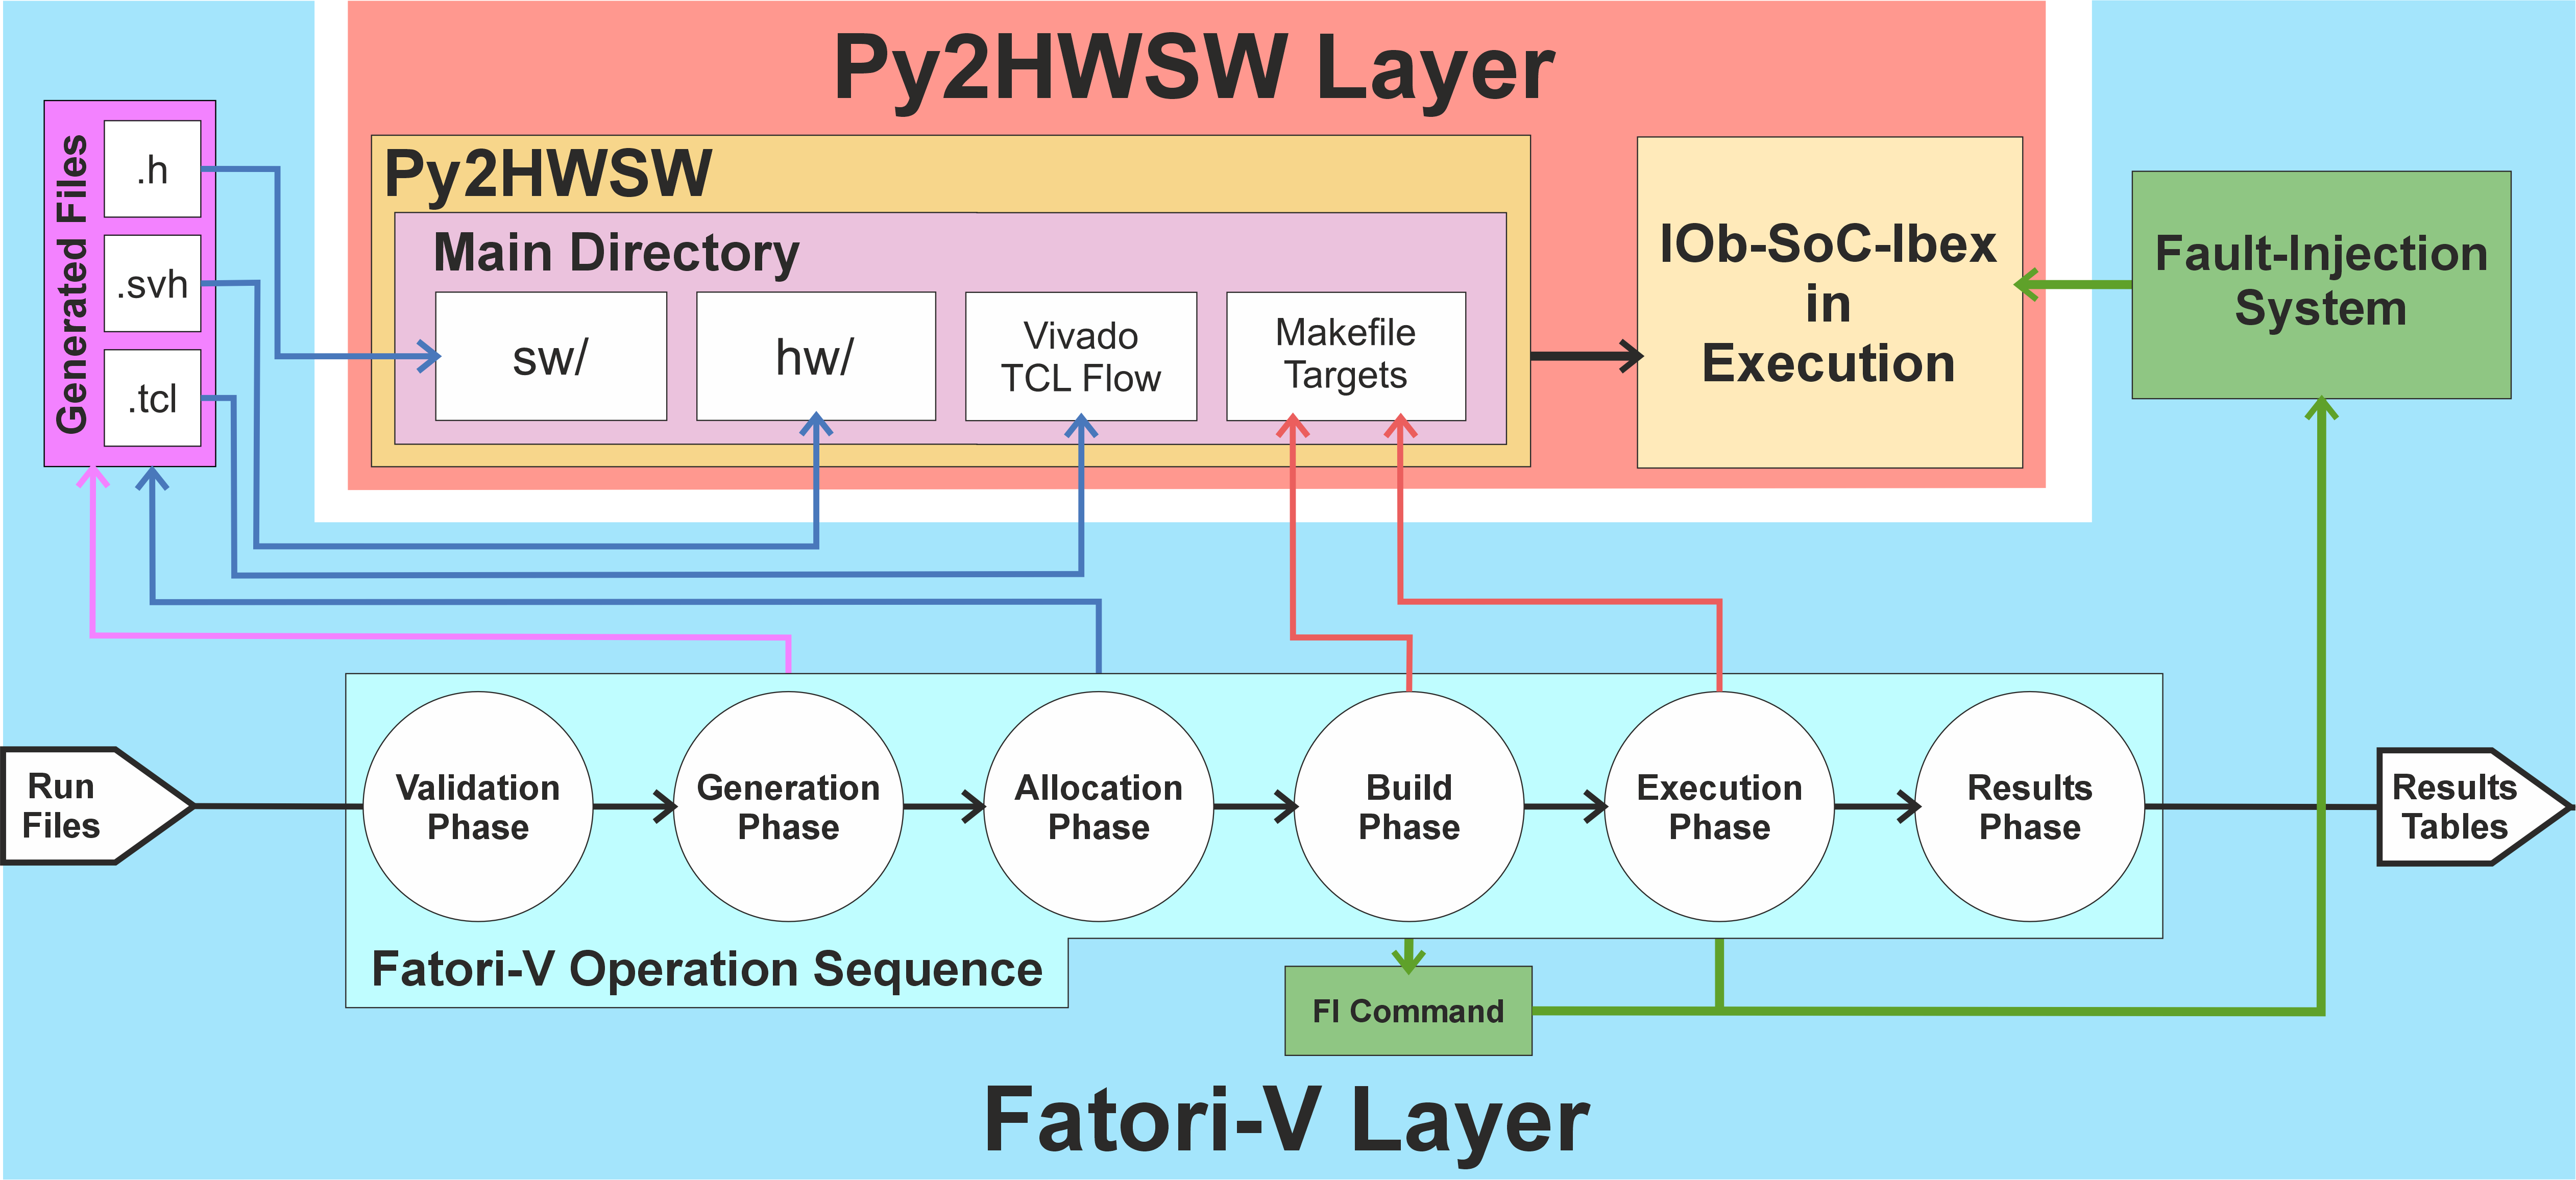
\includegraphics[width=0.9\textwidth]{Images/chap3_layers.png}
    \caption{\ac{Fatori-V} run flow from input run files to result tables.}
    \label{fig:fatori_overview}
\end{figure}


A \ac{Fatori-V} run starts from a user-defined \texttt{.yaml} file provided through \texttt{runs/}. Each run file describes the hardware configuration, benchmark setup, build options, and \ac{FI} parameters. The top script, \texttt{fatori-v.py}, reads the selected run files and executes the same staged workflow for each one, as shown in \Cref{fig:fatori_overview}.

During a run, \ac{Fatori-V} validates the user configuration, generates the required interface files, stages those files in the architecture and benchmark repositories, builds the configured system, executes the selected benchmark sessions, and writes the final result tables. When \ac{FI} is enabled, the same flow also prepares the \ac{FI} command and launches the \ac{FI} tool during benchmark execution.

The Validation Stage checks the run \texttt{.yaml} before any file is generated. The checks are defined in \texttt{config/validation\_checks.py}. Each check inspects selected fields and either applies a deterministic correction or aborts the run. In strict mode, warnings without automatic corrections also abort the run. After validation, \ac{Fatori-V} writes \texttt{verified\_yaml.yaml}, which is used by the remaining stages and stored in the final results folder. Users can add custom checks to \texttt{config/validation\_checks.py}.

The Generation Stage translates the verified configuration into the interface macro files required by the build flow. These include SystemVerilog headers such as \texttt{fatori\_features.svh}, \texttt{fatori\_ftm.svh}, \texttt{fatori\_logic\_mon.svh}, \texttt{fatori\_reg\_mon.svh}, \texttt{fatori\_selftest.svh}, and \texttt{fatori\_pblocks.svh}. It also generates firmware headers for benchmark selection and Vivado \texttt{.tcl} scripts for the build flow.

The File Movement Stage copies generated files according to \texttt{gen\_locations.yaml}. User-provided hardware and software inputs are copied according to the corresponding \texttt{locations.yaml} files. Before overwriting a destination file, \ac{Fatori-V} creates a backup so the repository can be restored after the run.

The Build Stage runs the IOb-\ac{SoC}-Ibex Makefile targets. It builds the \ac{FPGA} image, prepares the selected benchmarks, and stores the implementation reports used later for hardware metrics. When \ac{FI} is enabled, this stage also prepares the \ac{FI} command used during execution.

The Execution Stage runs each enabled benchmark as a separate session. A session is valid when the process exits cleanly, the benchmark succeeds, and a valid \texttt{metrics.txt} file, containing measured data, is produced. When \ac{FI} is enabled, the session controller launches the \ac{FI} tool as a parallel process and uses the synchronization mechanism described in \Cref{chap7:sw_logging}.

The Results Stage collects the session data, benchmark outputs, \texttt{metrics.txt} files, \ac{FI} logs, and implementation reports. These files are stored under \texttt{results/} and used to create the result tables.






% #############################################################################
\section{Pblock Sizing Model}
\label{chap7:pblock}

To inject faults into a specific hardware module, the \ac{FI} tool must know where that module is placed in the \ac{FPGA}. \ac{Fatori-V} solves this by constraining each injectable target to a pblock and storing its bounds in the System Dictionary used by the \ac{FI} tool. These bounds are later used to select configuration memory addresses that belong to the target region, as described in \Cref{chap8:fi_acme_impl}.

The size of each hardware module depends on the active Ibex configuration, including \ac{ISA} extensions, multiplier type, bit manipulation variant, cache support, branch logic, writeback stage, \ac{FI} instrumentation, and enabled \acp{FTM}. A static table would not cover all possible combinations, especially for parameters such as the M-of-N replication factor, which can be virtually any integer number. The Pblock Sizing Model estimates the required area of each target from the configuration used in each run.

The model is used for the following pblock targets: \ac{ALU}, \ac{LSU}, Controller, Decoder, IF Stage, ID Stage, Multiplier, Prefetch Buffer, WB Stage, Branch Predictor, and Fault Manager.







% -----------------------------------------------------------------------------
\subsection{Sizing Equations}
\label{chap7:pblock_sizing_model}

The model estimates the \ac{LUT} and \ac{FF} usage of each pblock target. Each target starts from a measured baseline and adds the overhead of the active hardware features. The baseline with architectural features is defined in \Cref{eq:pblock_target_base}.

\begin{equation}
A_t =
B_t
+
\sum \Delta^{\text{feat}}_t
\label{eq:pblock_target_base}
\end{equation}

In \Cref{eq:pblock_target_base}, \(B_t\) is the measured \ac{LUT} baseline of target \(t\), and \(\sum \Delta^{\text{feat}}_t\) is the sum of the enabled architectural feature overheads. Negative feature effects are set to zero, preventing the model from estimating  pblock sizes below the measured baseline.

Logic M-of-N replicates the complete target. This includes the combinational logic and the registers inside the target. Register M-of-N overhead, if the \ac{FTM} is enabled, is included within each logic replica. The \ac{LUT} estimate is computed with \Cref{eq:pblock_lut_model}.

\begin{equation}
\text{LUT}_t =
N_{\text{logic}}
\left(
A_t
+
\Delta^{\text{RegMon}}_t(N_{\text{reg}})
\right)
+
V_t(N_{\text{logic}})
\label{eq:pblock_lut_model}
\end{equation}

In \Cref{eq:pblock_lut_model}, \(N_{\text{logic}}=1\) when Logic M-of-N is disabled. \(V_t(N_{\text{logic}})\) is the voter cost of the Logic M-of-N wrapper and is set to zero when Logic M-of-N is disabled.

Register M-of-N mainly increases the number of \acp{FF}, because it replicates stored state. However, the generated wrappers, voters, correction logic, and control logic can also use \acp{LUT}. For this reason, the model includes a Register M-of-N \ac{LUT} term when measured data showed a relevant \ac{LUT} cost. This term is computed with \Cref{eq:pblock_reg_mon}.

\begin{equation}
\Delta^{\text{RegMon}}_t(N_{\text{reg}})
=
P_t(N_{\text{reg}})
-
A_t
\label{eq:pblock_reg_mon}
\end{equation}

In \Cref{eq:pblock_reg_mon}, \(P_t(N_{\text{reg}})\) is the measured or fitted total \ac{LUT} count of target \(t\) with Register M-of-N enabled. When Register M-of-N is disabled, or when the measured \ac{LUT} overhead was not relevant, \(\Delta^{\text{RegMon}}_t(N_{\text{reg}})=0\).

The \ac{FF} model follows the same structure. The model starts from the measured \ac{FF} baseline, adds the \ac{FF} effects of the enabled architectural features, and applies the \ac{FF} cost of Register M-of-N when enabled. Since XCKU040 slices contain 8 \acp{LUT} and 16 \acp{FF}, the final pblock size is set by the most restrictive resource, as shown in \Cref{eq:pblock_slice_binding}.

\begin{equation}
\text{Slices}_{t}
=
\left\lceil
M_t
\cdot
\max
\left(
\left\lceil \frac{\text{LUT}_{t}}{8} \right\rceil,
\left\lceil \frac{\text{FF}_{t}}{16} \right\rceil
\right)
\right\rceil
\label{eq:pblock_slice_binding}
\end{equation}

\(M_t\) is the safety margin used to account for placement and routing constraints. 





% -----------------------------------------------------------------------------
\subsection{Measured Model Parameters}
\label{chap7:pblock_study}

The model parameters were extracted from implementation reports generated for the XCKU040 \ac{FPGA}. Each experiment enabled a controlled hardware configuration, implemented the design, and parsed the utilization reports to measure the \ac{LUT} and \ac{FF} usage of each pblock target.

The experiments were organized to isolate the terms defined in \Cref{eq:pblock_target_base,eq:pblock_lut_model,eq:pblock_reg_mon}. Baseline experiments measured each target with optional features and \acp{FTM} disabled. Feature experiments enabled one parameter at a time, including RV32B, RV32M, instruction cache, branch prediction, branch target \ac{ALU}, and writeback stage. M-of-N experiments varied \(N\) for Logic M-of-N and Register M-of-N. Combined experiments checked whether the extracted terms still produced usable pblock sizes when features and \acp{FTM} were enabled together.

\Cref{tab:pblock_feature_params} reports the baseline and feature parameters used in \(A_t\). RV32M values are ordered as none, single-cycle, fast, and slow. RV32B values are ordered as none, balanced, full, and OTEarlGrey. Empty entries mean that no positive measured contribution was kept.

\begin{table}[h]
\centering
\scriptsize
\setlength{\tabcolsep}{2.8pt}
\renewcommand{\arraystretch}{1.20}
\begin{tabularx}{\textwidth}{|X|X|X|X|X|}
\hline
\rowcolor{tableheader}\textbf{Target} &
\textbf{Baseline} &
\textbf{RV32M \(\Delta\ac{LUT}\)} &
\textbf{RV32B \(\Delta\ac{LUT}\)} &
\textbf{Notes} \\
\hline
\hline
\ac{ALU} &
96 \acp{LUT}, 0 \acp{FF} &
0, 7, 10, 51 &
0, 27, 27, 29 &
Pure \ac{ALU} has no registers. \\
\hline
Multiplier &
0, 326, 317, 357 \acp{LUT}; 0, 74, 75, 76 \acp{FF} &
Set by RV32M mode &
 &
DSP count is also stored per RV32M mode. \\
\hline
Controller &
331 \acp{LUT}, 14 \acp{FF} &
0, 10, 1, 51 &
 &
RV32B effects are set to zero. \\
\hline
Decoder &
257 \acp{LUT}, 1 \ac{FF} &
 &
0, 40, 38, 40 &
RV32M has no measured effect. \\
\hline
\ac{LSU} &
103 \acp{LUT}, 68 \acp{FF} &
0, 16, 9, 7 &
0, 45, 42, 44 &
Used by load/store logic. \\
\hline
IF Stage &
1667 \acp{LUT}, 284 \acp{FF} &
0, 305, 235, 361 &
0, 930, 1802, 1750 &
Largest feature variation. \\
\hline
ID Stage &
334 \acp{LUT}, 17 \acp{FF} &
0, 5, 32, 97 &
0, 0, 86, 0 &
\ac{FF} effects are also fitted. \\
\hline
WB Stage &
135 \acp{LUT}, 75 \acp{FF} &
 &
 &
Only when enabled. \\
\hline
Prefetch Buffer &
486 \acp{LUT}, 199 \acp{FF} &
0, 0, 13, 0 &
 &
Disabled when instruction cache is enabled. \\
\hline
Branch Predictor &
38 \acp{LUT}, 0 \acp{FF} &
 &
 &
Only when enabled. \\
\hline
Fault Manager &
5 \acp{LUT}, 114 \acp{FF} &
 &
 &
Metrics included. \\
\hline
\end{tabularx}
\caption{Baseline and feature parameters used by the Pblock Sizing Model.}
\label{tab:pblock_feature_params}
\end{table}

\Cref{tab:pblock_redundancy_params} reports the redundancy parameters used after \(A_t\) is computed. Logic M-of-N terms are used inside \Cref{eq:pblock_lut_model}. Register M-of-N terms are used to compute \(\Delta^{\text{RegMon}}_t(N_{\text{reg}})\) in \Cref{eq:pblock_reg_mon}.

\begin{table}[h]
\centering
\scriptsize
\setlength{\tabcolsep}{2.8pt}
\renewcommand{\arraystretch}{1.22}
\begin{tabularx}{\textwidth}{|p{0.16\textwidth}|p{0.38\textwidth}|p{0.30\textwidth}|X|}
\hline
\rowcolor{tableheader}\textbf{Target} &
\textbf{Logic M-of-N \ac{LUT} term} &
\textbf{Register M-of-N term} &
\textbf{Notes} \\
\hline
\hline
\ac{ALU} &
\((N_{\text{logic}}-1)A_{\text{ALU}} + 26.63N_{\text{logic}}^2 + 1249.09N_{\text{logic}} - 97.21\) &
0 &
No registers. \\
\hline
Controller &
\(30N_{\text{logic}}^2 + 800N_{\text{logic}}\) &
\(P(N_{\text{reg}})=70.38N_{\text{reg}}+68.03\), \(\text{FF}=15N_{\text{reg}}\) &
Register term is inside each logic replica. \\
\hline
Decoder &
\((N_{\text{logic}}-1)A_{\text{DEC}} + 1594N_{\text{logic}}\) &
\(\text{FF}=N_{\text{reg}}\) &
One baseline \ac{FF}. \\
\hline
\ac{LSU} &
\((N_{\text{logic}}-1)A_{\text{LSU}} + 89.61N_{\text{logic}}^2 - 645.61N_{\text{logic}} + 1609.00\) &
\(P(N_{\text{reg}})=280.47N_{\text{reg}}-510.13\), \(\text{FF}=66N_{\text{reg}}+2\) &
Fitted from register runs. \\
\hline
IF Stage &
\((N_{\text{logic}}-1)A_{\text{IF}} + 23.93N_{\text{logic}}^2 - 1860.13N_{\text{logic}} + 2164.80\) &
\(P(N_{\text{reg}})=1465.65N_{\text{reg}}-548.46\), \(\text{FF}=321N_{\text{reg}}\) &
Fitted from register runs. \\
\hline
ID Stage &
Logic Redundancy not implemented &
\(P(N_{\text{reg}})=367.97N_{\text{reg}}-441.69\), \(\text{FF}=87N_{\text{reg}}\) &
No standalone Logic M-of-N target. \\
\hline
Prefetch Buffer &
Logic Redundancy not implemented &
\(\text{FF}=199N_{\text{reg}}\) &
Only without instruction cache. \\
\hline
\end{tabularx}
\caption{Redundancy parameters used by the Pblock Sizing Model.}
\label{tab:pblock_redundancy_params}
\end{table}

Negative measured contributions are kept at zero. This prevents synthesis optimizations from reducing the predicted pblock size below the measured baseline. The slice conversion from \Cref{eq:pblock_slice_binding} is applied after the \ac{LUT} and \ac{FF} estimates are computed.





% #############################################################################
\section{Benchmark Porting}
\label{chap7:benchmarks}

\ac{Fatori-V} integrates four benchmark programs that can run sequentially in the same experiment. These are IObundle's Hello World, CoreMark, Embench-IoT, and Fatori Stress. Hello World is used as a simple execution check. CoreMark and Embench-IoT provide standard performance benchmarks. Fatori Stress was developed in this work as a checksum-based way to evaluate \ac{FT} on Ibex.

All benchmarks were ported following the same folder structure under \texttt{benchmarks/}. Each benchmark has one folder whose name matches the key used in the run \texttt{.yaml}. The folder requires a \texttt{benchmark.h} file that defines \texttt{BENCHMARK\_MAIN} as the benchmark's main function, a \texttt{repo/} folder with the upstream source when applicable, a \texttt{Makefile} that generates the sources from \texttt{repo/}, and wrapper files that adapt the benchmark to the bare-metal firmware environment. Some benchmarks also include \texttt{requirements.yaml} to declare extra compile or link flags.

Benchmark options exposed by each port are routed to the run \texttt{.yaml}, so the user can configure benchmark parameters together with the remaining experiment settings.




% -------------------------------------------------------------
\subsection{CoreMark Benchmark}
\label{chap7:coremark}

CoreMark is included as a reference benchmark for comparing \ac{CPU} implementations. In \ac{Fatori-V}, the number of iterations is selected in the run \texttt{.yaml} file and compiled into \texttt{bench\_config.h} as \texttt{ITERATIONS}.

CoreMark evaluates linked-list handling, matrix operations, state-machine execution, and \ac{CRC} computation. The benchmark reports execution time, iteration count, iterations per second, memory configuration, and \ac{CRC} values. \ac{Fatori-V} parses these fields from the CoreMark report and stores them in \texttt{metrics.txt}. The CoreMark score is computed as the number of completed iterations divided by the measured execution time.

The port uses the official \texttt{core\_portme.c/h} files. The header selects static memory through \texttt{MEM\_STATIC} and disables floating-point support through \texttt{HAS\_FLOAT}. The source file redirects \texttt{ee\_printf} to the local print implementation.

The wrapper \texttt{coremark\_main.c} adapts the upstream entry point to the common benchmark interface. It renames CoreMark's original main function before including the upstream \texttt{core\_main.c}, allowing the firmware wrapper to call it through \texttt{BENCHMARK\_MAIN}. The files \texttt{coremark\_metrics.c/h} capture the CoreMark report, extract the relevant fields, and write them to \texttt{metrics.txt}.






% -------------------------------------------------------------
\subsection{Embench-IoT Benchmark}
\label{chap7:embench-iot}

Embench-IoT executes a set of embedded sub-benchmarks sequentially and combines their results into a score commonly used to evaluate \acp{CPU}. In \ac{Fatori-V}, the user selects the enabled sub-benchmarks through the run \texttt{.yaml} file. This selection is compiled into \texttt{bench\_config.h}, with one enable macro per sub-benchmark.

Each selected Embench-IoT sub-benchmark prepares its input data, runs the timed benchmark code, and checks whether the produced output is correct. \ac{Fatori-V} records the executed sub-benchmarks, pass count, Embench-IoT score, cycle count, pass flag, and ratio between the measured cycle count and the reference cycle count stored in \texttt{embench\_data.h}. Because the software memory available on the board used in this work is limited, \ac{Fatori-V}'s validation restricts each run to ten enabled sub-benchmarks. If the run file enables more than ten, the excess entries are disabled before the build. This limit is defined in \texttt{validation\_checks.py}.

The file \texttt{embench\_benchmarks.c} includes the selected Embench-IoT programs and renames their \texttt{main} functions to avoid symbol conflicts. The file \texttt{embench\_main.c} runs each enabled sub-benchmark, measures cycles with \texttt{mcycle} and \texttt{mcycleh}, verifies the result, computes the ratio, and writes the measured values to \texttt{metrics.txt}. The files \texttt{boardsupport.c/h} provide the platform hooks required by Embench-IoT, and \texttt{requirements.yaml} adds the \texttt{-lm} link flag required by math-based sub-benchmarks.






% -------------------------------------------------------------
\subsection{Fatori Native Benchmark}
\label{chap7:fatori_stress}

Fatori Stress was developed in this work to provide a deterministic workload for \ac{FI} campaigns. It is self-validating and can be configured to exercise specific Ibex targets.

The benchmark executes the selected workload twice. The first pass runs from iteration \(0\) to \(N-1\). The second pass runs from iteration \(N-1\) back to \(0\). Each iteration computes a value from the iteration index and XORs it into a running checksum. Since XOR is self-inverse, a fault-free execution returns to the initial checksum after the backward pass. If a fault changes the computed values, the final checksum does not match and the benchmark reports \texttt{FAIL}.

The generated \texttt{bench\_config.h} file configures the benchmark. The macro \texttt{FATORI\_ITERATIONS} sets \(N\), and one macro per target selects which stress functions are executed. The current implementation supports the \ac{ALU}, Multiplier/Divider, Decoder, Controller, \ac{LSU}, Branch Predictor, and Instruction Decompressor.

Each iteration calls a dispatcher that executes the enabled target workloads and combines their return values into the checksum. The \texttt{alu\_stress} function exercises arithmetic, logic, shifts, and signed and unsigned comparisons. The \texttt{multiplier\_stress} function uses multiplication and division when RV32M is enabled, and uses software fallback loops otherwise. The \texttt{decoder\_stress} function alternates instruction formats through register-register operations, immediate operations, and volatile memory accesses. The \texttt{controller\_stress} function exercises control flow through nested conditions, loops, and non-inlined helper calls. The \texttt{lsu\_stress} function writes a known pattern to a static buffer and reads it back using byte, halfword, and word accesses. The \texttt{branch\_predict\_stress} function produces branch patterns. The \texttt{compressed\_stress} function is used when RV32C is enabled, forcing the instruction stream to include mixed 16-bit and 32-bit encodings.

During execution, Fatori Stress records the enabled target list, iteration count, initial checksum, forward checksum, backward checksum, validation status, and first mismatch iteration when a mismatch is detected.


% -------------------------------------------------------------
\section{Synchronization, Logging and Metrics Computing}
\label{chap7:sw_logging}

\ac{Fatori-V} synchronizes the \ac{FI} campaign with benchmark execution using a file-based handshake. Before starting the benchmark, the firmware running on the board requests the host \ac{PC} to create a synchronization file containing \texttt{WAIT}. The \ac{FI} tool receives the path to this file, waits until it is created, and writes \texttt{READY} when it is ready to inject. The firmware polls the same file and starts the benchmark only after reading \texttt{READY}.

The firmware and the \ac{FI} tool complete their setup before the synchronization step, so the benchmark and the campaign can start immediately after the handshake. The firmware initializes the \ac{UART}, samples the pre-benchmark metrics, prepares the benchmark, and writes \texttt{WAIT}.

A small timing offset can still exist. The \ac{FI} tool starts the campaign after writing \texttt{READY}, while the firmware only observes that update on its next polling iteration. A short delay is inserted after synchronization, but the first injections may still occur slightly before the benchmark begins executing. The experiments use large injection pools, so this offset has limited impact on the final campaign statistics.

Logging is centralized through the event system under \texttt{scripts/logging/}. Scripts do not print messages directly. They emit a log event with an event identifier and the fields needed to build the message. The logger then decides whether the event is printed and how it is formatted.

Logging can be tuned through two configuration files. \texttt{log\_levels.py} defines which events are shown for each verbosity level, and \texttt{messages\_formats.py} defines the corresponding message text. This lets users control how much information \ac{Fatori-V} reports during a run, while keeping prefixes, timestamps, terminal output, and log files consistent across the platform.


\ac{Fatori-V} generates result tables using measured and computed values. During the Results Stage, it loads \texttt{config/metrics\_definitions.py}, computes every defined metric for each benchmark session, and adds the values to the output tables. Users can extend this file with new metrics. Metrics measured in hardware are called direct metrics and must be written by the firmware to \texttt{metrics.txt}. Once defined, direct metrics can be used to compute indirect metrics, if their formulas are added to \texttt{config/metrics\_definitions.py}.

Some direct metrics are sampled before and after the benchmark. For these metrics, the firmware writes both values to \texttt{metrics.txt}, and \ac{Fatori-V} stores the post-minus-pre difference in the result tables.

The Results Stage also parses Vivado implementation reports to add hardware metrics. The final tables combine direct metrics, indirect metrics, benchmark-specific fields, \ac{FI} metrics, and implementation data. \Cref{app_b:metrics} lists the metrics exported by \ac{Fatori-V} in its current version.



% #############################################################################
\section{Summary}
\label{chap7:summary}

This chapter presented the campaign orchestration component of the Fatori-V layer. The operation sequence was described, showing how \ac{Fatori-V} translates \texttt{.yaml} run files into configured hardware and software builds and drives the full experiment lifecycle. The Pblock Sizing Model was presented, enabling module-targeted configuration memory injections. Benchmark porting was described for CoreMark, Embench-IoT, and the Fatori Native benchmark. Finally, the synchronisation, logging, and metrics infrastructure was presented, covering the file-based handshake, the event-driven logging system, and the result-table generation pipeline. \Cref{chap8:fatori_fi} describes the fault injection tool, also part of this layer.


